\documentclass[border=0.125in]{standalone}
 
% Bar chart drawing library 
\usepackage{pgfplots} 
\usetikzlibrary{patterns}
 
\begin{document}
 
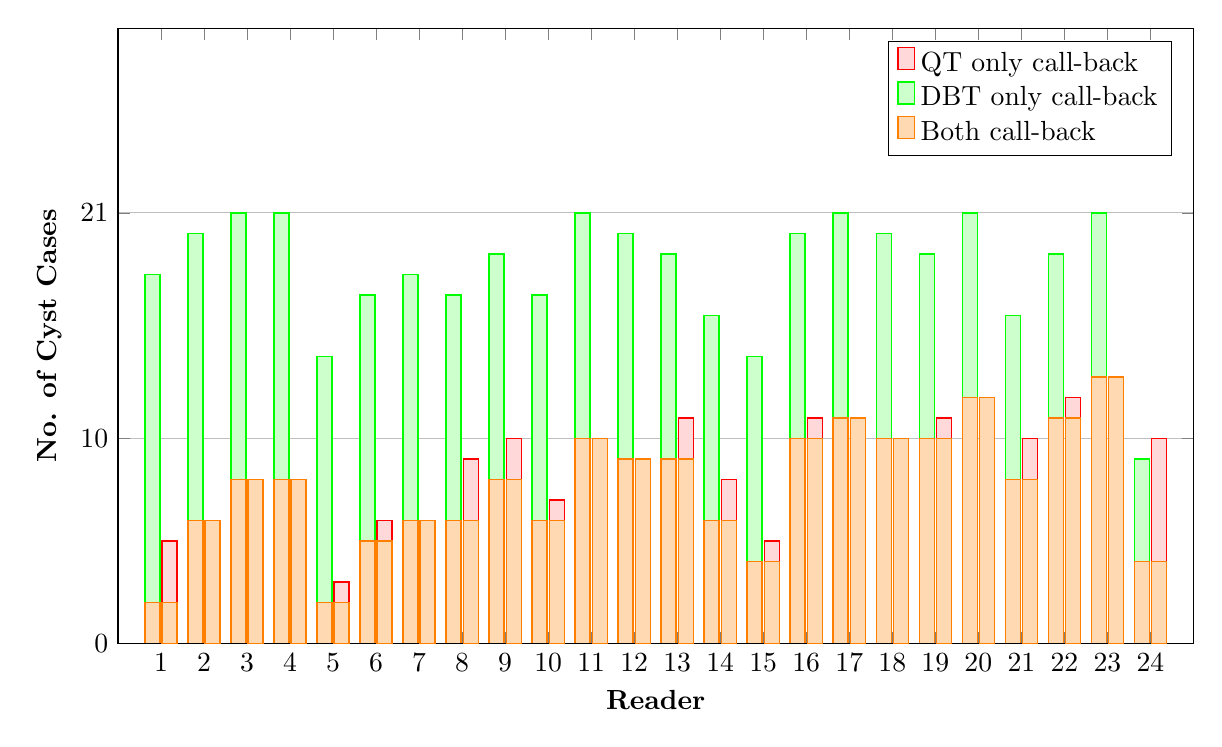
\begin{tikzpicture}
 
\begin{axis} [ybar stacked,
	width = 6in,
	height = 3.7in,
    bar width = 8pt,
    xmin = 0,
    xmax = 25,
    ymin = 0,
    ymax = 30,
%    xtick = {},
    xtick = {1,2,3,4,5,6,7,8,9,10,11,12,13,14,15,16,17,18,19,20,21,22,23,24},
    ytick = {0,10,21},
    ymajorgrids = true,
%    ytick = data,
	xlabel = {\textbf{{Reader}}},
	ylabel = {{\textbf{{No. of Cyst Cases}}}},
	legend cell align={left},
	reverse legend,
%    enlarge x limits = {abs = .05, },
%    enlarge y limits = {abs = .8}
]

% BothMQ
\addplot+ [draw = orange,
    line width = .5pt,
    fill = orange!30,
%    fill opacity=0.4,
	bar width=.075in,
] coordinates {
(10.8, 10)
(4.8, 2)
(11.8, 9)
(18.8, 10)
(2.8, 8)
(23.8, 4)
(6.8, 6)
(8.8, 8)
(5.8, 5)
(13.8, 6)
(1.8, 6)
(21.8, 11)
(16.8, 11)
(7.8, 6)
(3.8, 8)
(15.8, 10)
(9.8, 6)
(17.8, 10)
(22.8, 13)
(14.8, 4)
(19.8, 12)
(20.8, 8)
(.8, 2)
(12.8, 9)
};
 
 % MGonly
 \addplot+ [draw = green,
    line width = .5pt,
    fill = green!20,
%    fill opacity=0.7,
%    pattern = dots,
%    pattern color = blue
	bar width=.075in,
]   coordinates {
(10.8, 11)
(4.8, 12)
(11.8, 11)
(18.8, 9)
(2.8, 13)
(23.8, 5)
(6.8, 12)
(8.8, 11)
(5.8, 12)
(13.8, 10)
(1.8, 14)
(21.8, 8)
(16.8, 10)
(7.8, 11)
(3.8, 13)
(15.8, 10)
(9.8, 11)
(17.8, 10)
(22.8, 8)
(14.8, 10)
(19.8, 9)
(20.8, 8)
(.8, 16)
(12.8, 10)
};

 % QTonly
\addplot+ [draw = red,
    line width = .5pt,
    fill = red!15,
%    fill opacity=0.4,
	bar width=.075in,
] coordinates {
(-10,10)
};

\legend {Both call-back, DBT only call-back, QT only call-back};

\end{axis}

 
% % NeitherMQ
%\addplot+ [draw = blue,
%    line width = .5pt,
%    fill = blue!7,
%%    fill opacity=0.4,
%] coordinates {
%(11, 0)
%(5, 6)
%(12, 1)
%(19, 1)
%(3, 0)
%(24, 6)
%(7, 3)
%(9, 0)
%(6, 3)
%(14, 3)
%(2, 1)
%(22, 1)
%(17, 0)
%(8, 1)
%(4, 0)
%(16, 0)
%(10, 3)
%(18, 1)
%(23, 0)
%(15, 6)
%(20, 0)
%(21, 3)
%(1, 0)
%(13, 0)
%};
 
 
\begin{axis} [ybar stacked,
	width = 6in,
	height = 3.7in,
    bar width = 8pt,
    xmin = 0,
    xmax = 25,
    ymin = 0,
    ymax = 30,
%    xtick = {},
    xtick = {1,2,3,4,5,6,7,8,9,10,11,12,13,14,15,16,17,18,19,20,21,22,23,24},
    ytick = {0,10,21},
    xtick = \empty,
    ytick = \empty,
%	xlabel = {\textbf{{Reader}}},
%	ylabel = {{\textbf{{No. of Cancer Cases}}}},
	legend cell align={left},
	reverse legend,
%    enlarge x limits = {abs = .05, },
%    enlarge y limits = {abs = .8}
]

% BothMQ
\addplot+ [draw = orange,
    line width = .5pt,
    fill = orange!30,
%    fill opacity=0.4,
	bar width=.075in,
] coordinates {
(11.2, 10)
(5.2, 2)
(12.2, 9)
(19.2, 10)
(3.2, 8)
(24.2, 4)
(7.2, 6)
(9.2, 8)
(6.2, 5)
(14.2, 6)
(2.2, 6)
(22.2, 11)
(17.2, 11)
(8.2, 6)
(4.2, 8)
(16.2, 10)
(10.2, 6)
(18.2, 10)
(23.2, 13)
(15.2, 4)
(20.2, 12)
(21.2, 8)
(1.2, 2)
(13.2, 9)
};
 
 % QTonly
\addplot+ [draw = red,
    line width = .5pt,
    fill = red!15,
%    fill opacity=0.4,
	bar width=.075in,
] coordinates {
(11.2, 0)
(5.2, 1)
(12.2, 0)
(19.2, 1)
(3.2, 0)
(24.2, 6)
(7.2, 0)
(9.2, 2)
(6.2, 1)
(14.2, 2)
(2.2, 0)
(22.2, 1)
(17.2, 0)
(8.2, 3)
(4.2, 0)
(16.2, 1)
(10.2, 1)
(18.2, 0)
(23.2, 0)
(15.2, 1)
(20.2, 0)
(21.2, 2)
(1.2, 3)
(13.2, 2)
};
 
%\draw [line width=.25pt, color=black] (axis cs:0,0.0) -- (axis cs:25,0.0);

%\legend {Both call-back, Neither call-back, QT only call-back, DBT only call-back};
 
\end{axis}
 
\end{tikzpicture}
 
\end{document}
